
\newpage
\appendix
\section*{Appendix}
In support of the main paper,~\cref{app:proofs} presents the proofs for the propositions in the paper,~\cref{app:additional_findings} includes additional findings that support our main results, and~\cref{app:further_discussion} provides further discussion on conditions that lead to grokking.
\section{Proofs}\label{app:proofs}
\begin{proof}[Proof of~\cref{prop:stablemax}]
\begin{align}
    \softmax\left(g\left(x_i\right)\right) &= \frac{e^{g(x_i)}}{\sum_j e^{g(x_j)}}\\
    &= \begin{cases}
\frac{e^{\log(x_i+1)}}{\sum_j e^{\log(x_j+1)}} & \text{if } x_i \geq 0, \\
\frac{e^{-\log(-x_i+1)}}{\sum_j e^{-\log(-x_j+1)}} & \text{if } x_i < 0
\end{cases}\\
&= \begin{cases}
\frac{x_i+1}{\sum_j x_j+1} & \text{if } x_i \geq 0, \\
\frac{\frac{1}{-x_i+1}}{\sum_j \frac{1}{-x_j+1}} & \text{if } x_i < 0
\end{cases}\\
&= \stablemax(x_i).
\end{align}
\end{proof}

\begin{proof}[Proof of~\cref{prop:NLMGrad}]
To prove that any nonzero $-\nabla_{\perp} \loss(\bm{\theta}_t)$ is a descent direction, we need to show that $\left\langle -\nabla_{\perp} \loss(\bm{\theta}_t), \nabla\loss(\bm{\theta}_t) \right\rangle < 0$, assuming $\nabla_{\perp} \loss(\bm{\theta}_t) \neq \mathbf{0}$:
    \begin{equation}
        \left\langle \nabla\loss(\bm{\theta}_t), -\nabla\loss(\bm{\theta}_t) + \left( \frac{\bm{\theta}_t^\top \nabla \loss(\bm{\theta}_t)}{\bm{\theta}_t^\top \bm{\theta}_t} \right)\bm{\theta}_t  \right\rangle \leq 0.
    \end{equation}
    Expanding this yields:
    \begin{align}
        -\left\|\nabla\loss(\bm{\theta}_t)\right\|^2_2 + 
        \left\langle  \nabla\loss(\bm{\theta}_t), \bm{\theta}_t \frac{\bm{\theta}_t^\top \nabla \loss(\bm{\theta}_t)}{\bm{\theta}_t^\top \bm{\theta}_t}\right\rangle
        &\leq 0.
    \end{align}
    Since the inequality is unaffected by the scaling of the left hand side, we can, without loss of generality, assume that the gradients are normalized, leading to:
    \begin{align}\label{eq:incidence}
        \left\langle \nabla\loss(\bm{\theta}_t), \bm{\theta}_t \frac{\bm{\theta}_t^\top \nabla \loss(\bm{\theta}_t)}{\bm{\theta}_t^\top \bm{\theta}_t}\right\rangle
        &{\leq} 1.
    \end{align}
    Since $\bm{\theta}_t \frac{\bm{\theta}_t^\top \nabla \loss(\bm{\theta}_t)}{\bm{\theta}_t^\top \bm{\theta}_t}$ denotes the projection of the gradient onto the space spanned by the weights, $\langle\cdot,\cdot\rangle$ will measure the acute angle of incidence and hence~\cref{eq:incidence} holds, with equality iff $\nabla_{\perp} \loss(\bm{\theta}_t) = \mathbf{0}$, which is prevented by assumption. This proves that $-\nabla_{\perp} \loss(\bm{\theta}_t)$ is a descent direction while being perpendicular to the weights. %, the angle between $\loss(\bm{\theta}_t)$ and this projection will be the acute .
\end{proof}
We note that the \ograd stops when $\nabla_{\perp}\loss(\bm{\theta}_t) = \mathbf{0}$. If $\nabla\loss(\bm{\theta}_t) \neq \mathbf{0}$, this corresponds to the condition where the gradient is in the same direction with the parameter vector. $\nabla_{\perp}\loss(\bm{\theta}_t) = \mathbf{0}$ can also be the case if $\nabla\loss(\bm{\theta}_t) = \mathbf{0}$, which corresponds to the loss function being at a local optimum.

\section{Additional Findings}\label{app:additional_findings}


\subsection{Further evidence that SC prevents grokking} \label{app:sc_intervention}
\begin{wrapfigure}[12]{R}{0.38\textwidth}
            \vspace{-0.4cm}
            \begin{center}
    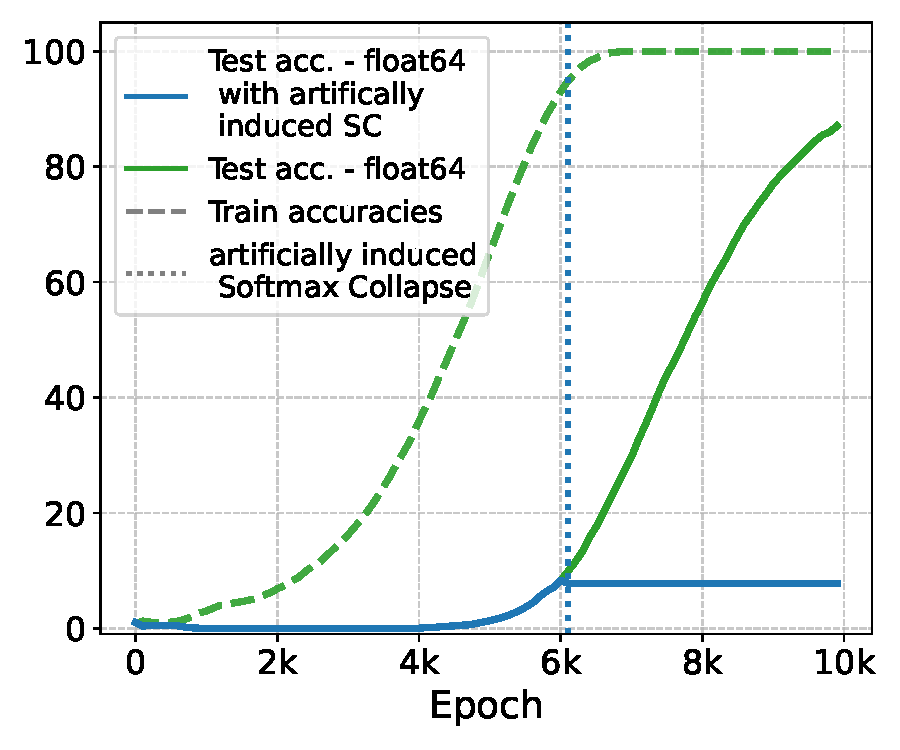
\includegraphics[width=\linewidth]{grokking_iclr_arxiv/figures/artificially_induced_sc.pdf}
            \end{center}
            \vspace{-12pt}
            \caption{Taking a model that would normally generalize (green) and artificially inducing SC has a very similar effect to the one observed in \cref{fig:grokking_stops}.\vspace{4mm}}
    \label{fig:sc_intervention}
\end{wrapfigure} 
While SC leads the gradient from correctly predicted samples to be zero, it does not do this for the incorrect classes. To validate that setting the gradients from the correct classes to zero is enough to stop learning, we do this artificially for a model that is generalizing and show that learning stops after this intervention. In \cref{fig:sc_intervention} we see that the baseline model shown in geen generalizes, but this is stopped at epoch 6000 for the model shown in blue, after we perform this intervention.

The intervention is implemented by multiplying the logits for the right classes by 0 at each step after epoch 6000.

\begin{comment}
\begin{figure}[h]
    \centering
    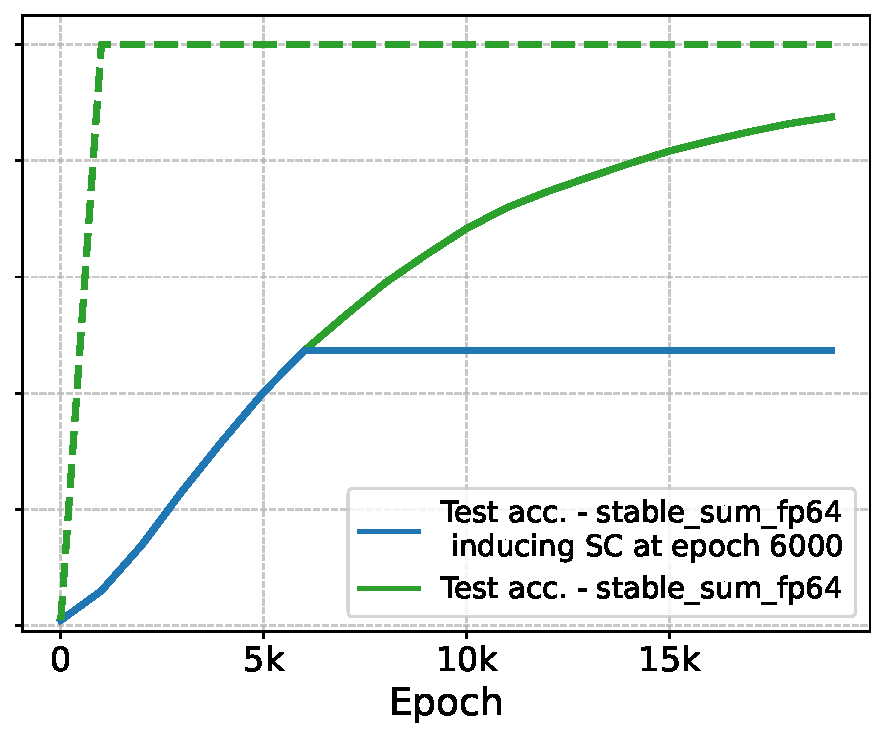
\includegraphics[width=0.5\linewidth]{grokking_iclr/figures/sc_intervention.pdf}
    \caption{Taking a model that would normally generalize (green) and artificially inducing SC has a very similar effect to the one observed in \cref{fig:grokking_stops}}.
    \label{fig:sc_intervention}
\end{figure}    
\end{comment}


\subsection{SGD with learning rate scheduling}
To show that our results are not due to the inductive bias of adaptive moments in optimizers like AdamW, we replicate some of the AdamW results using SGD with a learning rate scheduler. Our scheduler is similar to the one in \cite{Lyu2019-sc} except at each step we divide the learning rate by the norm of the full gradient, instead of the loss. In \cref{fig:grokking_stops_lr_sch} we observe that SC also puts an end to grokking in this setting.
\vspace{5.75mm}\\

\begin{figure}[t]
\centering
\begin{subfigure}{.32\textwidth}
  \centering
  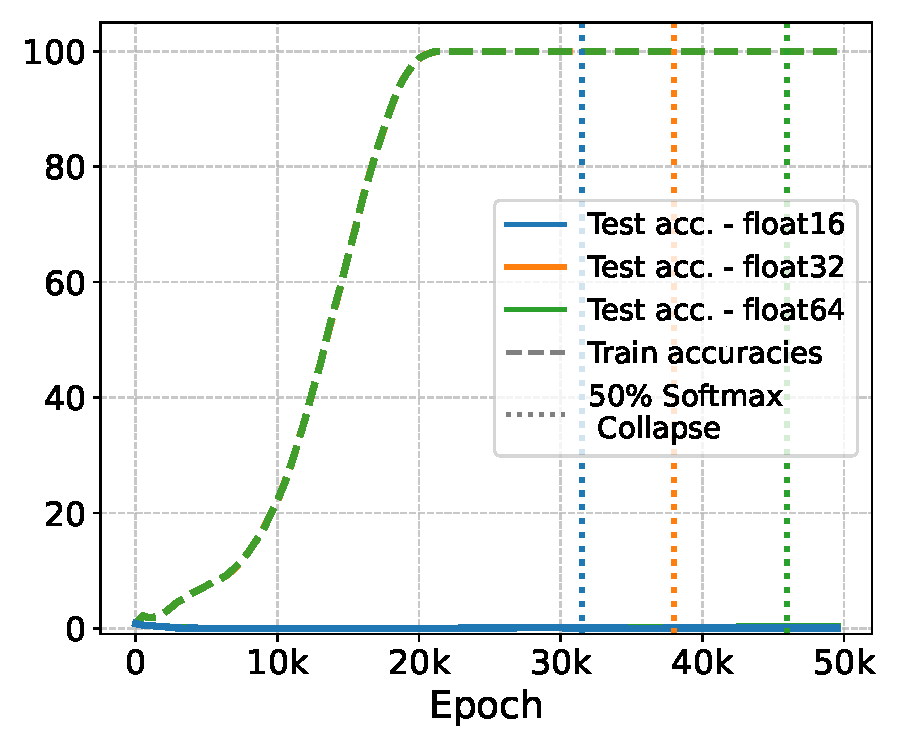
\includegraphics[width=\linewidth]{grokking_iclr_arxiv/figures/float32vsfloat64_40_percent_lr_sch.pdf}
  \caption{40\% training data}
  \label{fig:grokking_stops_40_lr_sch}
\end{subfigure}
\hfill
\begin{subfigure}{.32\textwidth}
  \centering
  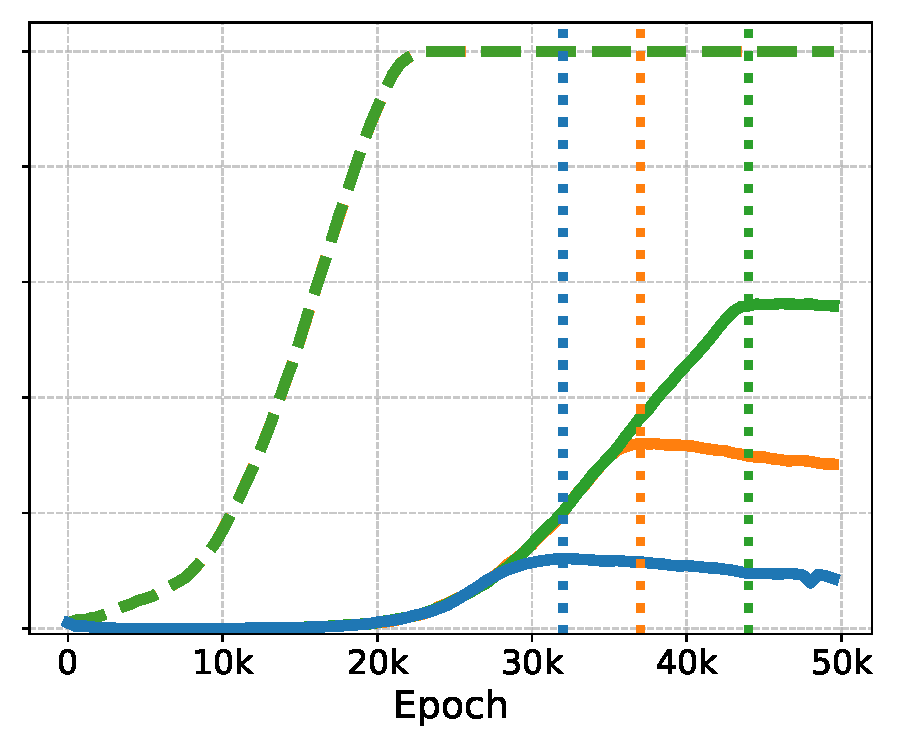
\includegraphics[width=\linewidth]{grokking_iclr_arxiv/figures/float32vsfloat64_60_percent_lr_sch.pdf}
  \caption{60\% training data}
  \label{fig:grokking_stops_60_lr_sch}
\end{subfigure}
\hfill
\begin{subfigure}{.32\textwidth}
  \centering
  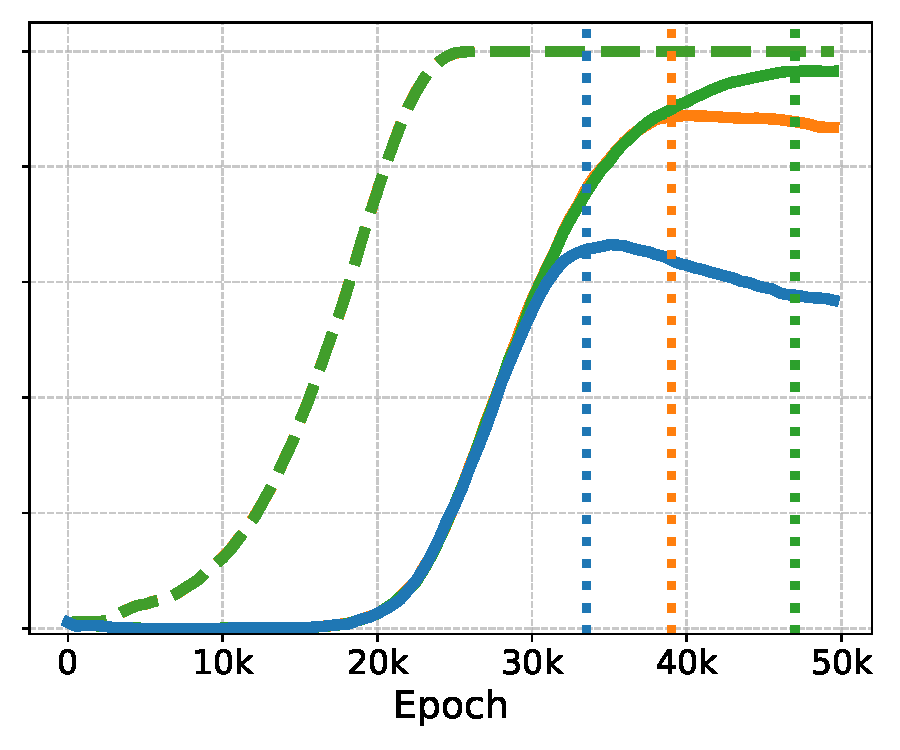
\includegraphics[width=\linewidth]{grokking_iclr_arxiv/figures/float32vsfloat64_70_percent_lr_sch.pdf}
  \caption{70\% training data}
\end{subfigure}
\caption{We show that the same dynamics observed in \cref{fig:grokking_stops} can be observed with a learning rate scheduler instead of AdamW. This shows that this is not due to an implicit bias of adaptive optimizers.}
\label{fig:grokking_stops_lr_sch}
\vspace{-5mm}
\end{figure}

\vspace{-5mm}
\section{Effective Learning Rate}
\begin{wrapfigure}[13]{R}{0.4\textwidth}
            \vspace{-1.2cm}
            \begin{center}
    \includegraphics[width=0.4\textwidth]{grokking_iclr_arxiv/figures/gradient_norms.pdf}
            \end{center}
            \vspace{-10pt}
            \caption{Gradient absorption errors during training on addition modulo 113.}
            \label{fig:gradient_absorption}
\end{wrapfigure} 
Unexplored in the main paper, NLM also has the effect of reducing the effective learning rate. For a gradient update using regular gradient descent $\bm{\theta}_{t+1} = \bm{\theta}_t - \eta \nabla \loss(\bm{\theta}_t)$ it is easy to see that $||\bm{\theta}_{t+1} - \bm{\theta}_{t}|| \to 0$ as $||\nabla \loss(\bm{\theta}_t)|| \to 0$. This problem has been observed before when training beyond the point of overfitting, for example, \cite{Lyu2019-sc} addressed it by using a loss based learning rate scheduler to keep up with the gradient. Theoretically, an alternative could be to simply extend the duration of training. According to our hypothesis, training for long enough should eventually lead to generalization on grokking tasks if we prevent SC. However, we find that another kind of floating point error can also appears in these settings, namely, gradient absorption errors in the weights. 

For a weight $w$, gradient absorption errors happen when a gradient update is small enough that it leaves the weight unchanged. Using the notation outlined in this paper this can be formalised as $w -\eta \frac{\partial \mathcal{L}}{\partial w} \doteq w$. In \cref{fig:gradient_absorption} we show that this happens for an MLP trained with SGD on modular addition using 30\% of the training data. As the norm of the gradient decreases, the percenage of the gradients that are absorbed by the weights increases substantially. Note that the number of gradients that are \textit{exactly} zero remains stable while the number of absorbed gradients increases substantially.

\begin{comment}
\begin{figure}[h]
    \centering
    \includegraphics[width=0.5\linewidth]{grokking_iclr/figures/gradient_norms.pdf}
    \caption{Gradient absorption errors during training on addition modulo 113.}
    \label{fig:gradient_absorption}
\end{figure}
\end{comment}
This issue is naturally mitigated by second order moments for adaptive optimizers like Adam and AdamW which is why they do not frequently appear. However, they do prevent us from showing grokking with vanilla gradient descent without any learning rate schduling. 


\subsection{Additional ways to induce grokking}
Beyond the interventions described in the main text, we highlight two additional ways to induce grokking that validate our hypothesis. 

\paragraph{Logit norm regularization}
Since we argue that uncontrolled scaling of the logits is responsible for delaying grokking and leading to SC, we validate that preventing this scaling of the logits by adding the norm of the logits to the loss, leads to grokking without additional regularization (\cref{fig:additional_grokking_logit}).


\begin{figure}[t]
\centering
\begin{subfigure}{.33\textwidth}
  \centering
  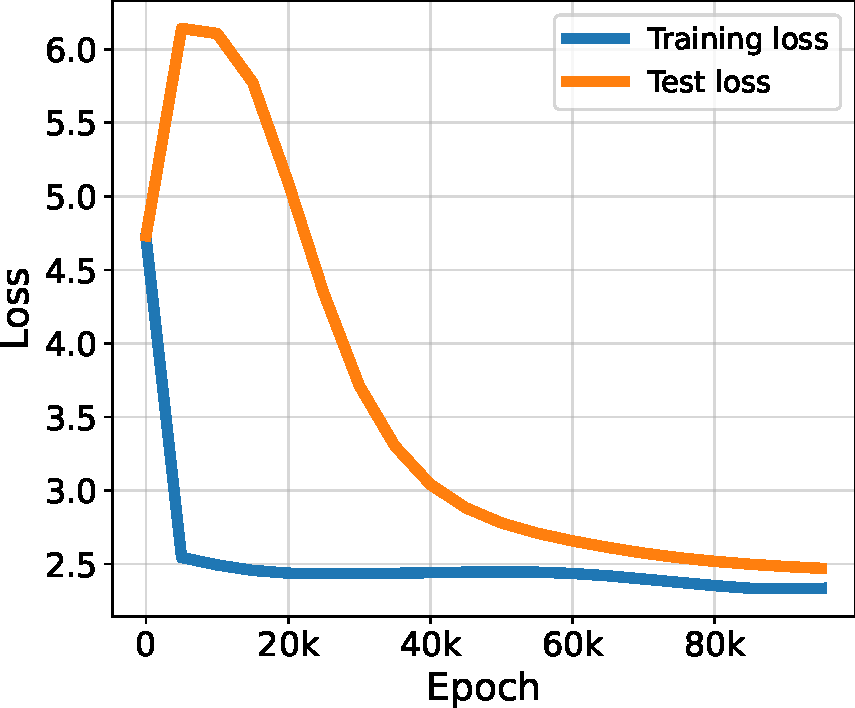
\includegraphics[width=\linewidth]{grokking_iclr_arxiv/figures/softermax_loss.pdf}
  \caption{$\stablemax$}
  \label{fig:additional_grokking_stablemax}
\end{subfigure}%
\hfill
\begin{subfigure}{.33\textwidth}
  \centering
  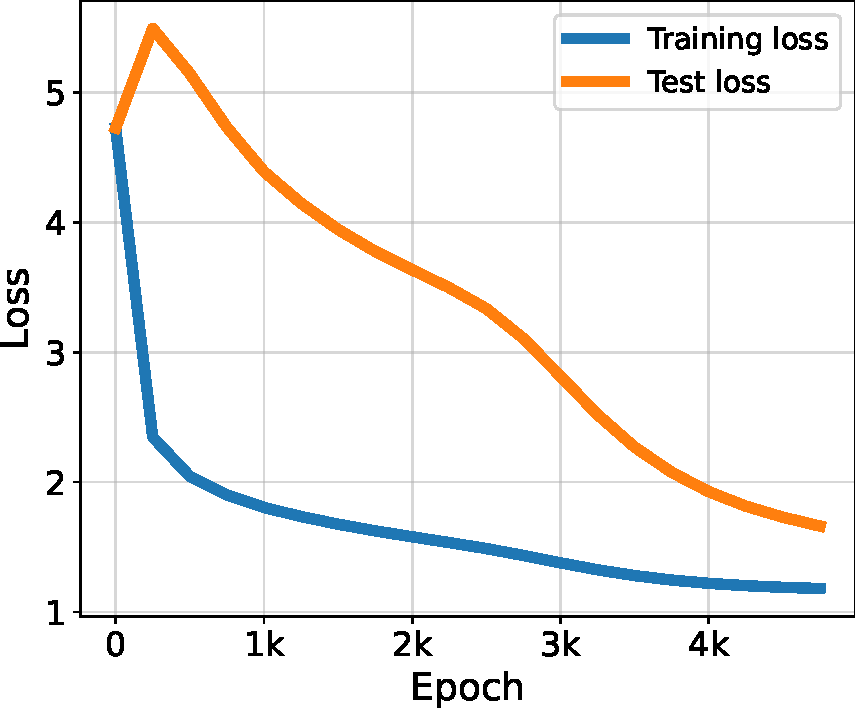
\includegraphics[width=\linewidth]{grokking_iclr_arxiv/figures/logit_reg_loss.pdf}
  \caption{Logit regularization}
  \label{fig:additional_grokking_logit}
  
\end{subfigure}%
\hfill
\begin{subfigure}{.33\textwidth}
  \centering
  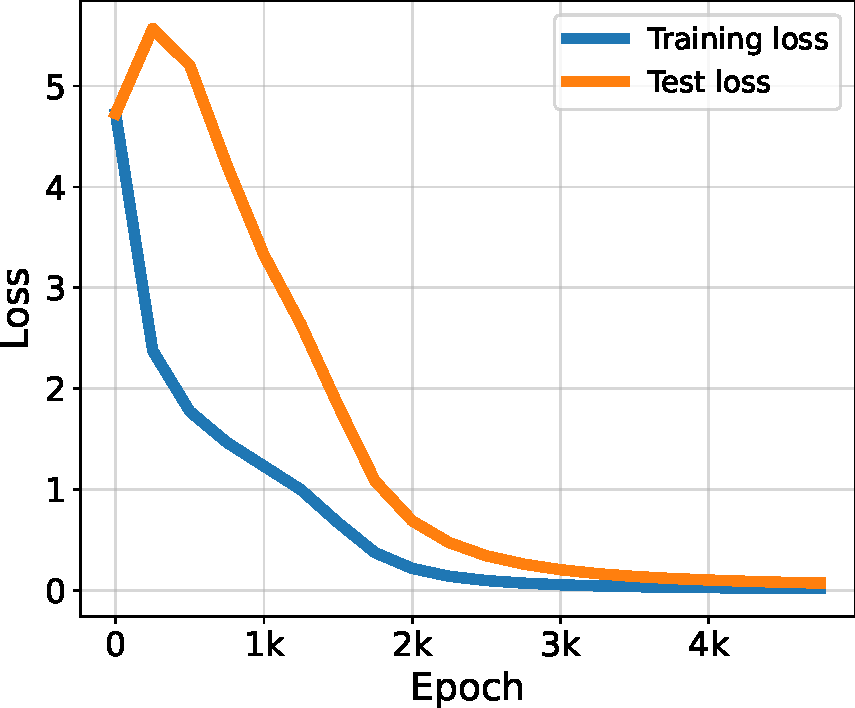
\includegraphics[width=\linewidth]{grokking_iclr_arxiv/figures/taylor_loss.pdf}
  \caption{\tsoftmax}
  \label{fig:additional_grokking_taylor}
\end{subfigure}
\vspace{-3mm}
\caption{Train and test losses during grokking induced by three different interventions.\vspace{-2mm}}
\label{fig:additional_grokking}
\end{figure}

\begin{wrapfigure}[20]{R}{0.4\textwidth}
\vspace{-0.5cm}
    \centering
    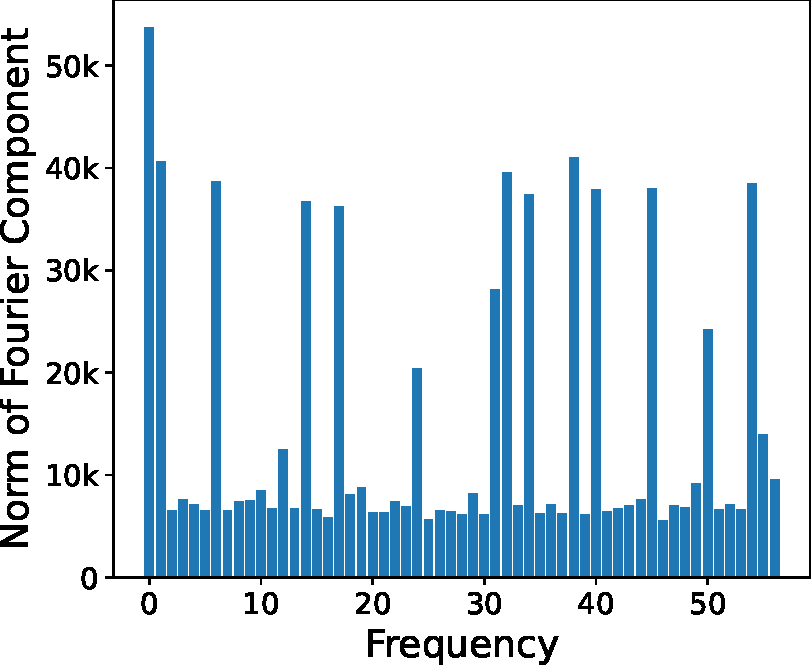
\includegraphics[width=\linewidth]{grokking_iclr_arxiv/figures/fourier.pdf}
    \vspace{-6mm}
    \caption{Fourier components of the weights of the output layer of an MLP trained on addition mod 113. Grokking is induced via $\stablemax$ and without weight decay.}
    \label{fig:fourier}
\end{wrapfigure}
\noindent\textbf{Taylor approximation of the Softmax.}
We have introduced $\stablemax$ as a change to the \softmax that leads to grokking without regularization. The motivation behind this is to prevent values in the sum of the \softmax that are very large or very close to zero. To this end, replacing the exponential with any function that is sub-exponential beyond a certain point should have a similar effect. To demonstrate, we perform a further experiment using the second order Taylor approximation of the exponential 
\begin{equation}
e^x\approx \frac{1 + x + x^2}{2!},    
\end{equation}
replacing the $\exp$ in the \softmax. Since the Taylor approximation is decreasing for $x<0$, we subtract the minimum logit to avoid this part of the function.  We deem this version \tsoftmax.
In \cref{fig:additional_grokking} we see results similar to the ones in \cref{fig:stablemax_grokking} but showing the losses instead of the accuracies as well as results for two additional methods to induce grokking. 
Note that our implementation of \tsoftmax (\cref{fig:additional_grokking_taylor}) introduces an additional implicit regularization similar to the one in  \cref{fig:additional_grokking_logit}, due to the gradient flowing through the subtraction of the mean. % also introduces an additional regularization effect similar to the one 
While this effectively combines the effects of \cref{fig:additional_grokking_stablemax} and \cref{fig:additional_grokking_logit}, leading to grokking faster than the other two methods, our main paper shows results using $\stablemax$ as a cleaner intervention that does not introduce this additional regularization effect. 

% above \tolga{what is the 'one above'?}. This is why we show our main results using $\stablemax$ as a cleaner intervention that does not introduce this additional regularization effect. 

%Note that our implementation of \tsoftmax (\cref{fig:additional_grokking_taylor}) introduces an implicit regularization similar to the one in  \cref{fig:additional_grokking_logit}, effectively combining the effects of \cref{fig:additional_grokking_stablemax} and \cref{fig:additional_grokking_logit}, explaining why it leads to grokking faster than the other two methods. 






\subsection{Solution Learned During Grokking  Without Weight Decay}\label{app:fourier}

\begin{comment}
    \begin{wrapfigure}[20]{R}{0.4\textwidth}
            \vspace{-0.5cm}
            \begin{center}
    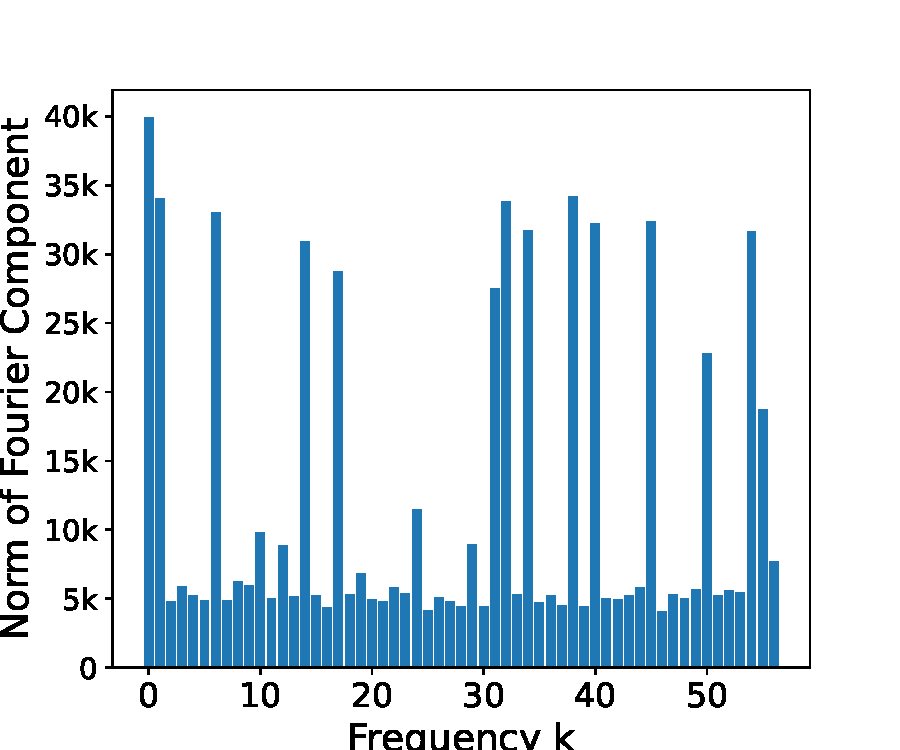
\includegraphics[width=0.4\textwidth]{grokking_iclr/figures/fourier_components.pdf}
            \end{center}
            \vspace{-10pt}
            \caption{Fourier components of the weights of the output layer of an MLP trained on addition mod 113. Grokking is induced with $\stablemax$ and without weight decay. \tolga{this figure is terribly cropped.}}
            \label{fig:fourier}
        \end{wrapfigure}
\end{comment}

 
Weight decay has been identified as potentially responsible for inducing the periodic structures in the weights studied in \cite{Nanda2023-hf}. In \cref{fig:fourier} we show that MLPs that grok without weight decay on modular addition show a similar sparsity in Fourier space as the one observed in \cite{Nanda2023-hf}. While these are very superficial results, they suggest that these structures can emerge without a weight decay--induced ``clean up'' phase as described in \cite{Nanda2023-hf}.

\section{Further Discussion on Conditions that Lead to Grokking}\label{app:further_discussion}
\subsection{L1 regularization and grokking}\label{app:l1_grokking}

%\paragraph{L1 regularization}
While it has been observed that L1 regularization can lead to grokking in some settings, \cite{Nanda2023-hf}
consistently found no grokking with L1 regularization and transformers and this setting has received substantially less attention than weight decay. 

We observe that \nlm scales the weights along their current direction. This means that larger weights are scaled more than small weights. However, while the sign of the gradient from L1 regularization depends on the sign of the weights, the magnitude of this gradient does not depend on the magnitude of the weights. This means that, particularly on deep networks or transformers with with large weights, L1 can sometimes be insufficient to prevent \nlm and the subsequent SC. 
%In Appendix \ref{app:l1_grokking} we show two examples, one where L1 regularization avoids SC and leads to grokking, and one where SC happens despite L1 regularization and grokking does not happen.

\subsection{Delaying generalization by scaling the weights} \label{app:scaling_weights}

\paragraph{Scaling the logits can delay generalization but not induce it} \cite{liu2023omnigrok}, \cite{Kumar2023-hz} and \cite{Lyu2023-ga} showed that an $\alpha$ parameter multiplying the logits can increase or reduce the delay in generalization. We highlight in \cref{fig:alpha_parameter} that this is true for cases where generalization happens even without changing the scale of the logits ($\alpha=1$). However, in most cases when using deeper networks or cross-entropy loss, models do not generalize by default without regularization and we are unable to induce grokking for any value of $\alpha$. 

We argue in \cref{sec:explain_existing_methods} that the observation in \cite{liu2023omnigrok}, \cite{Kumar2023-hz} and \cite{Lyu2023-ga} of grokking without regularization are due to the inductive bias of MSE loss which prevents NLM and leads to grokking in some settings for shallow networks.

\begin{figure}[t]
\centering
\begin{subfigure}{.33\textwidth}
  \centering
  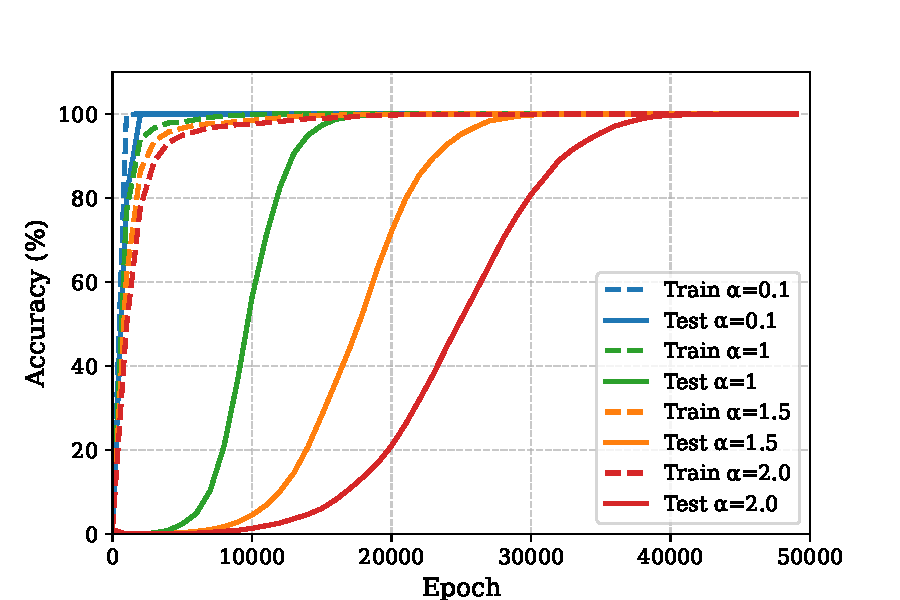
\includegraphics[width=\linewidth]{grokking_iclr_arxiv/figures/one_layer_MSE_alpha_sweep.pdf}
  \caption{MSE: 1 hidden layer}
\end{subfigure}%
\hfill
\begin{subfigure}{.33\textwidth}
  \centering
  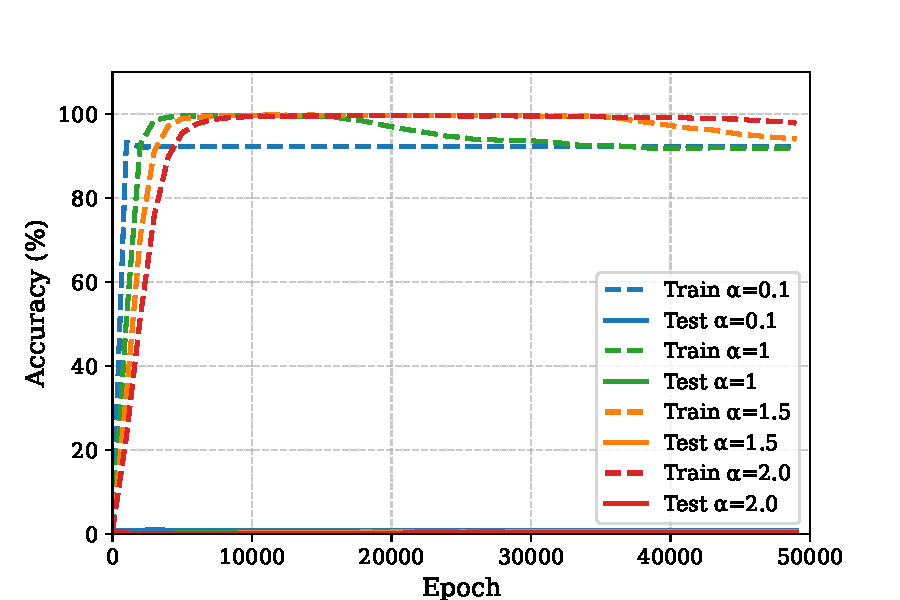
\includegraphics[width=\linewidth]{grokking_iclr_arxiv/figures/two_layer_MSE_alpha_sweep.pdf}
  \caption{MSE: 2 hidden layers}
\end{subfigure}%
\hfill
\begin{subfigure}{.33\textwidth}
  \centering
  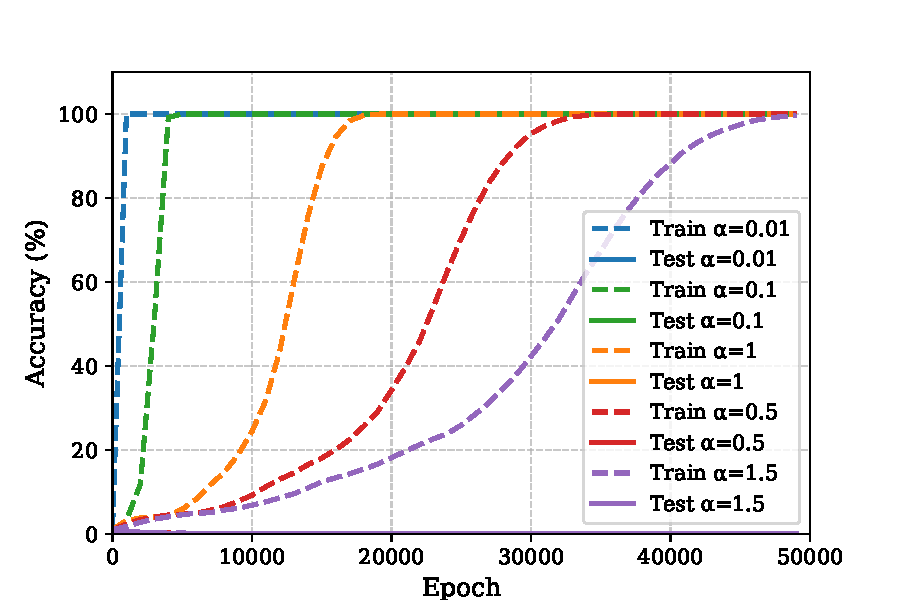
\includegraphics[width=\linewidth]{grokking_iclr_arxiv/figures/two_layer_cross_entropy_alpha_sweep.pdf}
  \caption{CE: 2 hidden layers}
\end{subfigure}
\caption{The $\alpha$ parameter controls generalization in settings where it happens by default. This is the case for shallow networks with MSE loss as shown in subplot (a). However, in deeper networks (b) or networks with CE loss and no regularization (c), $\alpha$ can control the time of over-fitting, but no value of $\alpha$ is enough to trigger grokking.}
\label{fig:alpha_parameter}
\end{figure}

\paragraph{Grokking on MNIST} We replicate the setting from \cite{liu2023grokking} of grokking on MNIST with cross-entropy loss and show that without weight decay, the scaling factor of the weights leads to significant FP errors, preventing grokking from happening until this is alleviated by weight decay. 

While SC explains why weight decay is needed to get the jump in performance observed in \cref{fig:mnist}. It could also explain why inducing grokking by scaling the weights is less effective when using SCE. While when using MSE loss, \cite{liu2023omnigrok} are able to induce full grokking from random level predictions to close to full training accuracy, the same does not seem to be possible when using SCE. In fact, we see in \cref{fig:mnist} that since the begining of training the rate of SC approaches 100\%. This could explain why the observations with cross-entropy loss are not the ones predicted by the lazy training theories outlined in \cite{Kumar2023-hz} which do not take limited floating point precision into account.

\begin{figure}[t]
    \vspace{-6mm}
    \centering
    \begin{subfigure}{.48\textwidth}
    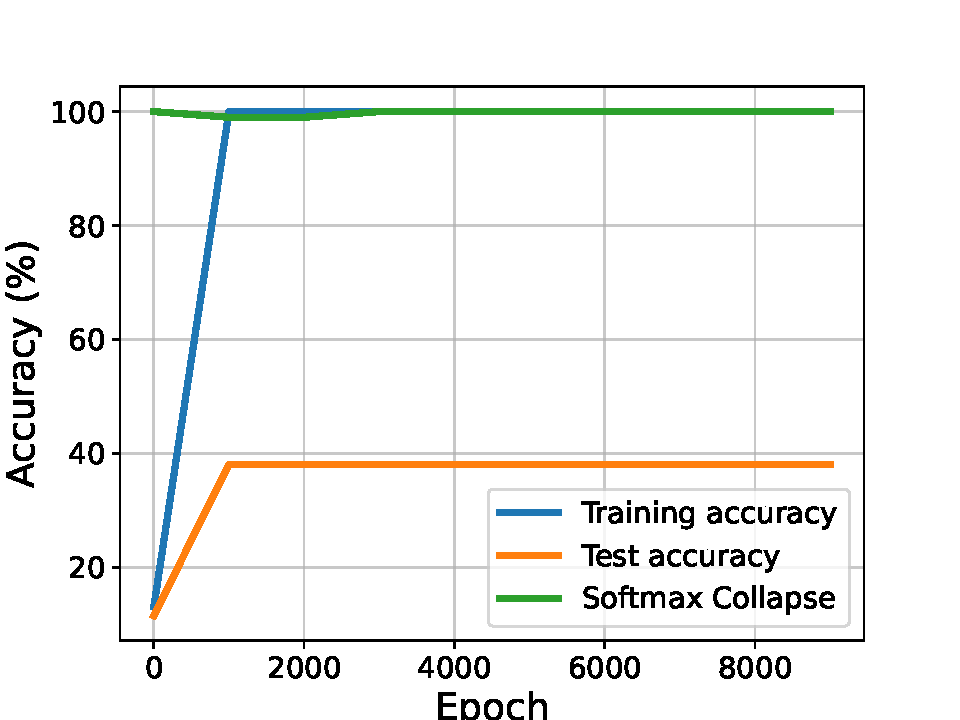
\includegraphics[width=\linewidth]{grokking_iclr_arxiv/figures/mnist_grokking.pdf}
        \caption{MLP without weight decay}
        \label{fig:mnist_witout_weight_decay}
    \end{subfigure}
    \begin{subfigure}{.48\textwidth}
    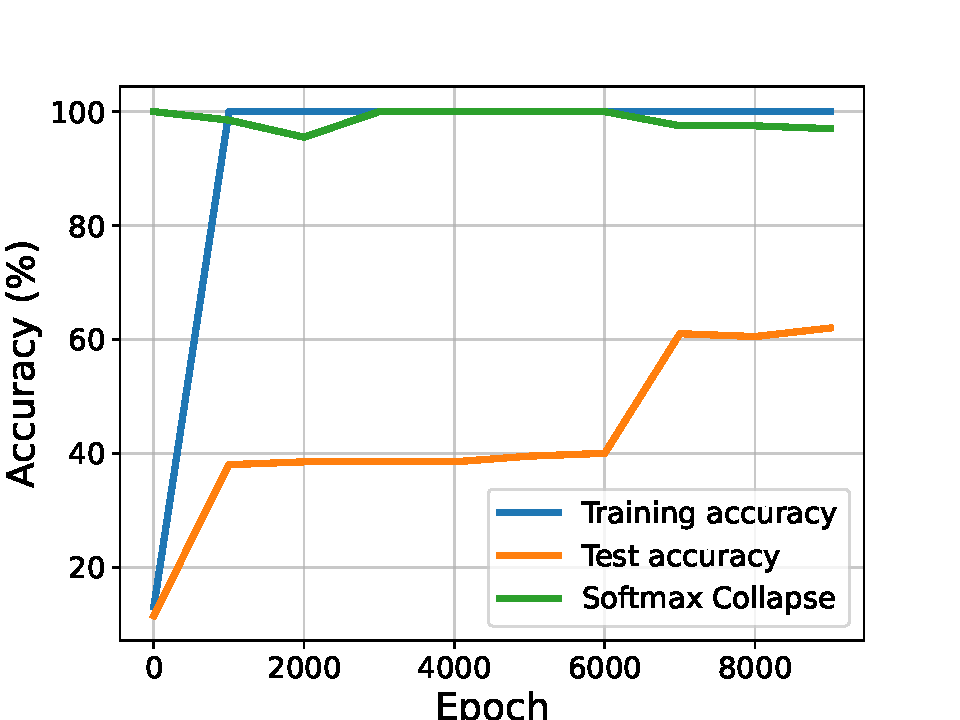
\includegraphics[width=\linewidth]{grokking_iclr_arxiv/figures/mnist_grokking_wd.pdf}
        \caption{MLP with weight decay.}
        \label{fig:mnist}
    \end{subfigure}
    \caption{Replicatting the grokking on MNIST for weight decay setting from \cite{liu2023grokking}. We find that MLPs with weights scaled up by 100 operate at the ``edge of numerical stability'' and in the absence of weight decay, SC eventually reaches 100\%, preventing any further generalization. When using weight decay, the weight norm is reduced, mittigating SC and eventually allowing for further generalization as the SC rate drops from 100\%.}

\end{figure}


\section{\ograd and Weight Decay}
In \cref{fig:wd_vs_ortho}, we provide a more in depth comparison of \ograd and weight decay. \cref{fig:wd_sweep} higlights that increasing the weight decay multiplier leads to a smaller delay in generalization, but only up to a point. In this concrete setting, a weight decay multiplier of 8, prevents the model from fully generalizing (\cref{fig:wd_sweep}). We then compare the best value of weight decay in this setting to \ograd, which does not require any hyper-parameter tuning. \cref{fig:vs_wd_seeds} shows that \ograd leads to faster grokking even when compared to a tuned value of weight decay. Note that the models with weight decay overfit immediately before grokking while \ograd reaches 100\% train and test accuracies almost at the same time.


\begin{figure}[t]
    \vspace{-5mm}
    \centering
    \begin{subfigure}{.48\textwidth}
    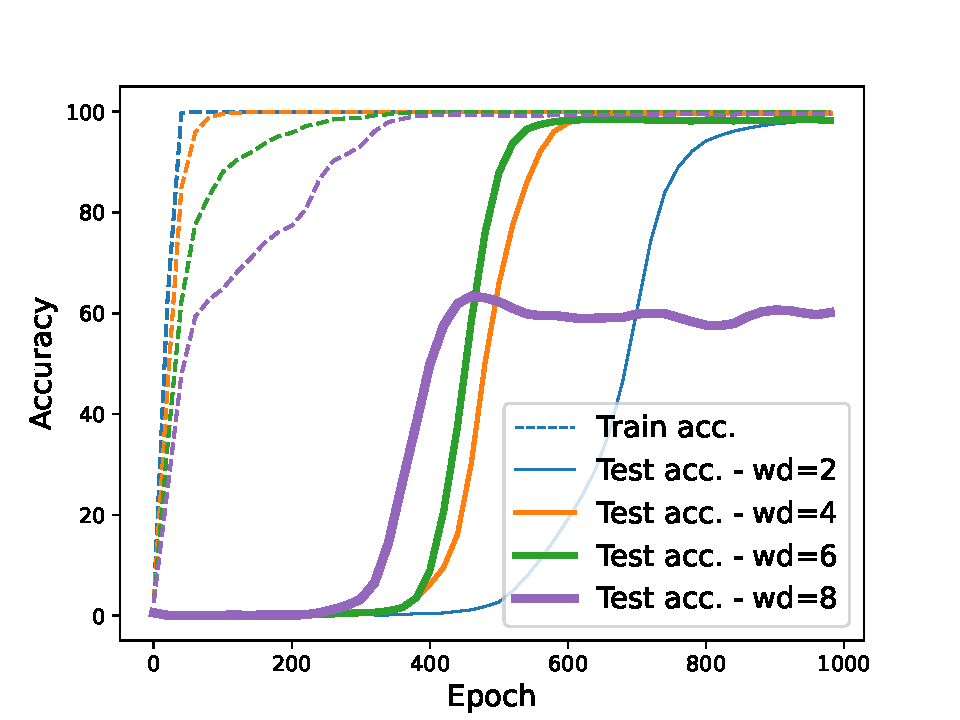
\includegraphics[width=\linewidth]{grokking_iclr_arxiv/figures/weight_decay_sweep.pdf}
        \caption{Sweep over values of weight decay}
        \label{fig:wd_sweep}
    \end{subfigure}
    \begin{subfigure}{.48\textwidth}
    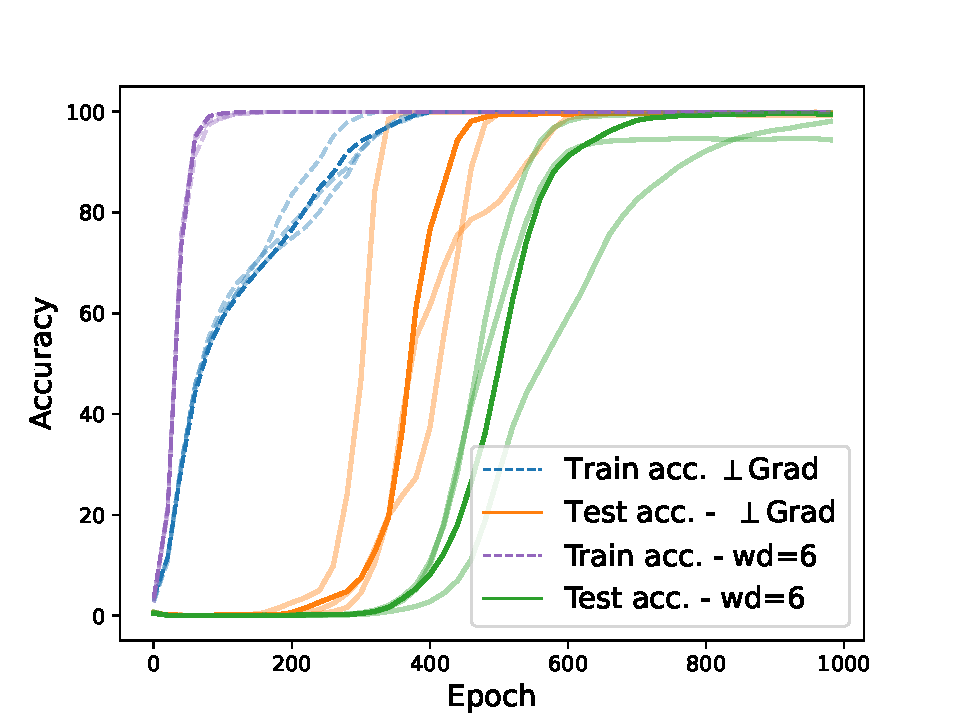
\includegraphics[width=\linewidth]{grokking_iclr_arxiv/figures/weight_decay_vs_orthograd_seeds.pdf}
        \caption{\ograd vs best performing wd model}
        \label{fig:vs_wd_seeds}
    \end{subfigure}
    \caption{Increasing weight decay (WD) for an MLP trained on modular addition with AdamW reduces the delay in generalization up to a point where WD prevents convergence \cref{fig:wd_sweep}. Without any tunable hyper-parameters and without WD, \ograd leads to grokking faster than the best model with WD \cref{fig:vs_wd_seeds}.}
    \label{fig:wd_vs_ortho}
\end{figure}

\section{Alternatives to $\stablemax$ in Preventing SC}
\begin{wrapfigure}[15]{R}{0.45\textwidth}
    \vspace{-7mm}
    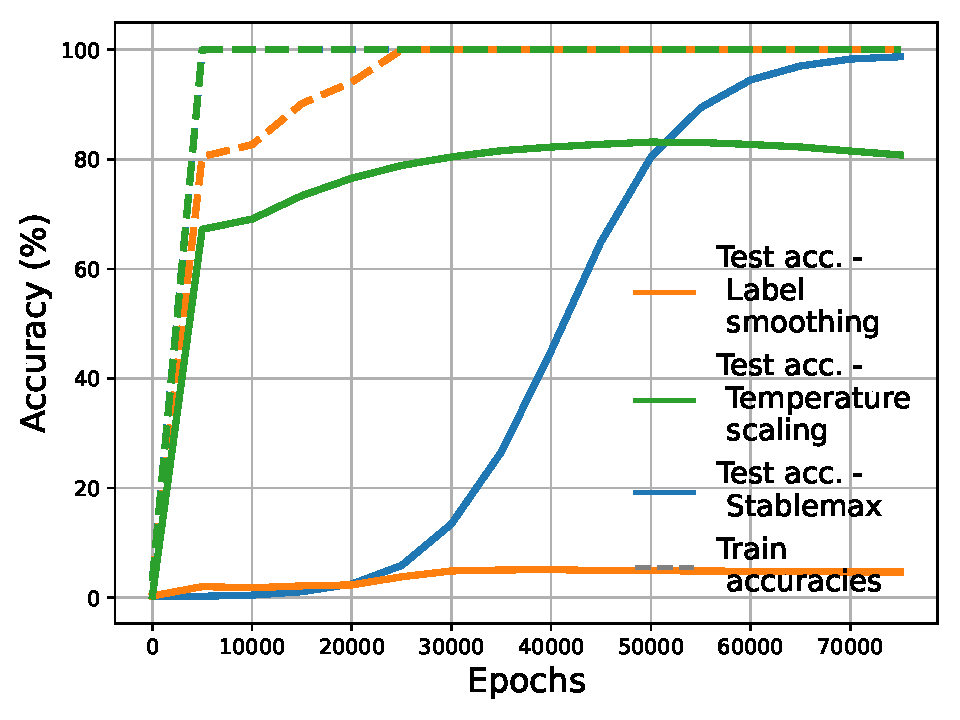
\includegraphics[width=\linewidth]{grokking_iclr_arxiv/figures/label_smoothing.pdf}
    \vspace{-8mm}
    \caption{$\stablemax$ prevents SC and leads to grokking while temperature scaling with $T=1e5$ only gradually delays SC, and label smoothing does prevent SC but at the cost of keeping the model from fully generalizing.}
    \label{fig:label_smoothing}
\end{wrapfigure}
While any intervention that prevents SC should lead to grokking or generalization, \cref{fig:label_smoothing} shows that scaling the temperature of the \softmax is not enough to prevent SC and label smoothing does prevent SC and lead to some generalization, but at the cost of introducing another inductive bias that prevents full generalization and leads to qualitatively different behavior. By comparison, the simple change introduced in Stablemax prevents SC and leads to grokking, serving as a validation for our hypothesis that gradient descent leads to grokking by default, unless this is stopped by SC.



\section{$\stablemax$ and \ograd \\ in Realistic Settings}
While Stablemax and \ograd are designed as interventions to show that preventing SC leads to grokking and preventing NLM leads to generalization (\cref{fig:teaser}), in this section we explore if these methods are applicable in more realistic settings like language modeling with GPT2-small or ResNets trained on image classification. We train GPT2-Small for 1 epoch on WikiText-103 using a batch size of 16, a block size of 512, a learning rate of $5e-4$ and a weight decay of 0.01 using AdamW. The architecture is the regular GPT2-Small architecture from \cite{radford2019language}, trained with a cosine schedule and 1000 steps of warmup.

For CIFAR10, CIFAR100 and Imagenet-1k \citep{ILSVRC15}, our baseline is a ResNet18 with SCE loss trained with SGD 0.9 momentum and $1e-4$ weight decay. We use standard data transformations such as random crop and random horizontal flip and a step learning rate scheduler every 30 epochs for a full training run of 100 epochs. With respect to this baseline we report results replacing the $\softmax$ with $\stablemax$ in the loss function, as well as replacing SGD with $\perp$SGD. Since test labels for Imagenet-1k are not publicly available, we use the validation set as a test set and tune hyper-parameters on a fraction of the training set.


\begin{figure}[t]
    \centering
    \begin{subfigure}{.32\textwidth}
    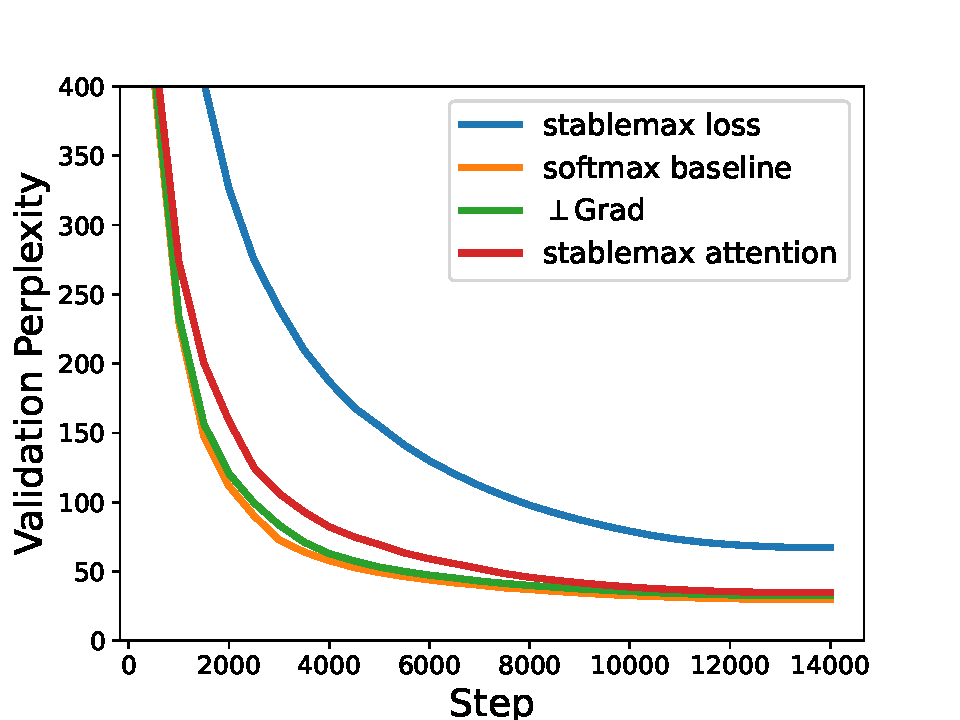
\includegraphics[width=\linewidth]{grokking_iclr_arxiv/figures/gpt2-small.pdf}
        \caption{GPT2-Small on WikiText2}
        \label{fig:gpt2_small}
    \end{subfigure}
    \hfill
    \begin{subfigure}{.32\textwidth}
    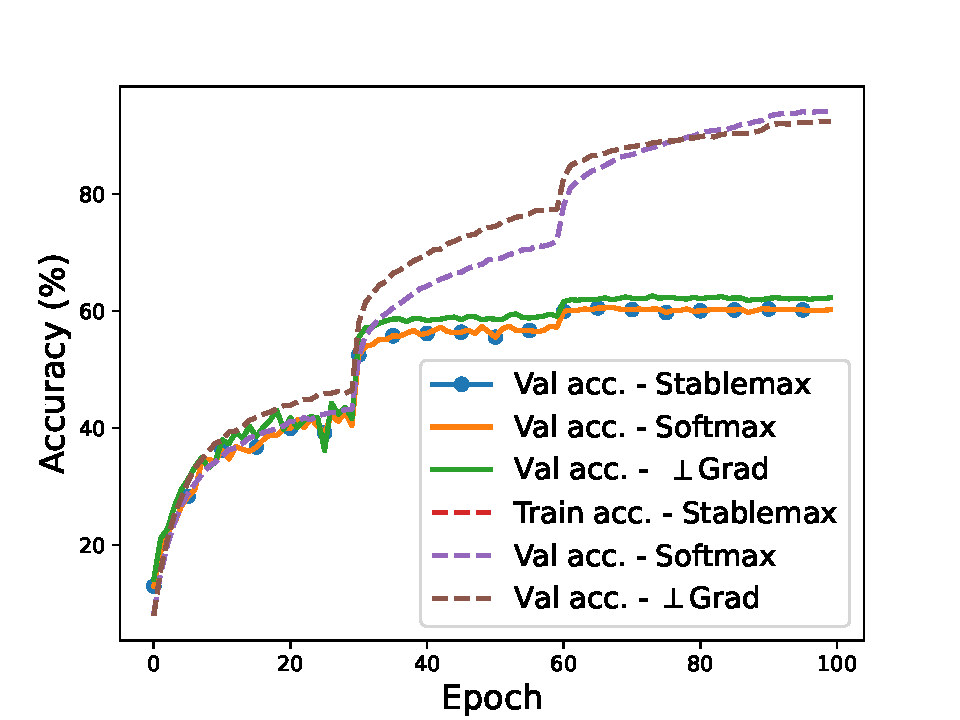
\includegraphics[width=\linewidth]{grokking_iclr_arxiv/figures/CIFAR100.pdf}
        \caption{ResNet18 on CIFAR100}
        \label{fig:cifar100_resnet18}
    \end{subfigure}
    \hfill
    \begin{subfigure}{.32\textwidth}
    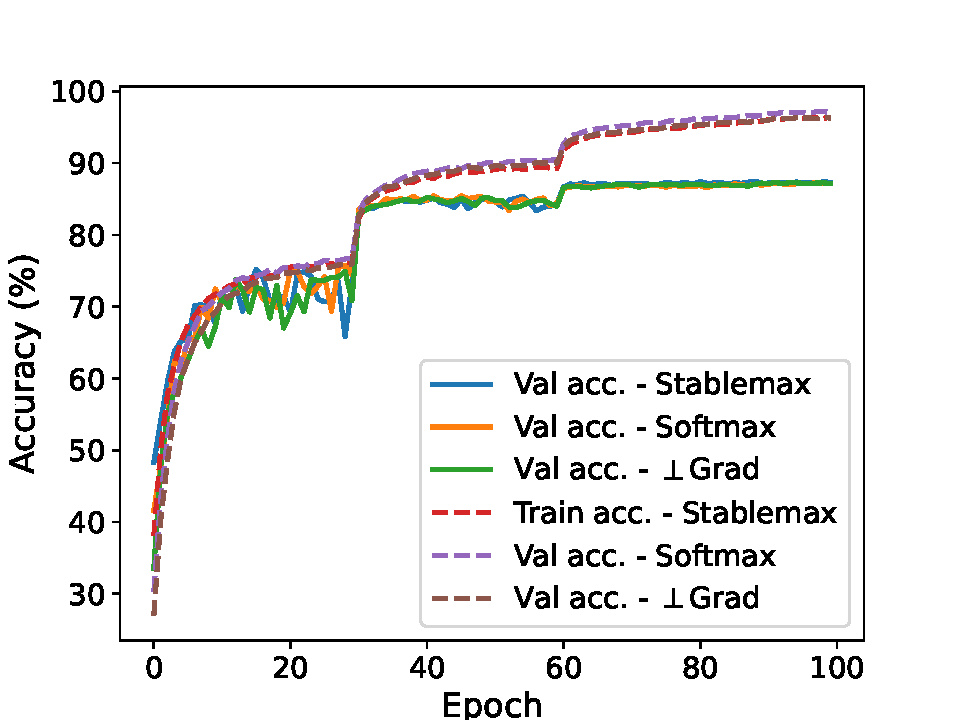
\includegraphics[width=\linewidth]{grokking_iclr_arxiv/figures/cifar10_resnet18.pdf}
        \caption{ResNet18 on CIFAR10}
        \label{fig:cifar10_resnet18}
    \end{subfigure}
    \caption{Comparing Stablemax and \ograd to AdamW with SCE on text data \cref{fig:gpt2_small} and image data \cref{fig:cifar10_resnet18}. For the GPT2-small results in \cref{fig:gpt2_small}, we also include the results of replacing the \softmax in the attention mechanism with $\stablemax$.}
\end{figure}

\begin{table}[h]
\centering
\begin{tabular}{@{}lcccc@{}}
\toprule
\textbf{Method}         & \textbf{CIFAR10} & \textbf{CIFAR100} & \textbf{ImageNet-1k} & \textbf{WikiText-103} (Top-5) \\ \midrule
Softmax CE              & $87.17\% \pm 0.2$ & $59.98\% \pm 0.4$  & $69.33\% \pm 0.04$              & $60.48\% \pm 0.04$                      \\
Stablemax CE            & $87.01\% \pm 0.2$ & $60.63\% \pm 0.4$  & $65.87\% \pm 0.22$             & $51.85\%  \pm 0.47$                  \\
\ograd                  & $87.22\% \pm 0.2$ & $62.69\% \pm 0.1$  & $68.95\% \pm 0.03$               & $59.64\%   \pm 0.04$                \\ 
\midrule
Stablemax Attention     & --                & --                 & --                   & $58.52\%   \pm 0.04$                   \\ \bottomrule
\end{tabular}
\label{tab:realistic_datasets}
\caption{For the methods introduced in this paper, we report accuracies with standard deviations across five seeds for the CIFAR datasets and three seeds for Imagenet-1k and WikiText-103. We report Top-5 accuracy in the case of WikiText-103.\vspace{-3mm}}
\end{table}


\section{SC and the Slingshot Effect}\label{app:slingshots}
\cite{slingshot-mechanism} observed that spikes in the training loss appear when training on grokking tasks with adaptive optimizers like Adam, and that these spikes can lead to generalization without weight decay. Although \cite{Nanda2023-hf} showed that slingshots are not necessary for grokking, it is still unclear what mechanism of adaptive gradient optimizers induces this behavior and why it leads to generalization. In light of the results in this paper, we believe that slingshots could lead to generalization because they prevent full SC. \cite{Nanda2023-hf} pointed out that something like SC could be responsible for these slingshots. One possible mechanism would be that zero gradients for some samples due to SC rapidly diminish the second-order moments leading to a large update or slingshot which moves the model away from full SC, although more research would be needed to properly show this.

While related to our work, slingshots are a different kind of instability which only appears with adaptive optimizers and can allow grokking. In contrast, we identify SC as a very specific issue in the \softmax that can affect any model trained with SCE, not only the ones trained with adaptive optimizers. Additionally SC prevents grokking whereas slingshots can lead to it. Wether and how slingshots are cause by SC remains an open research question, with some supporting evidence from \cite{Nanda2023-hf} which show that slingshots can disappear when using $float64$.

\section{Additional Details About Floating Points}
Beyond our main results, we found that in some cases, grokking could be stopped before SC due to the $\epsilon$ parameter in Adam being too large. While the $\epsilon$ term is designed to give numerical stability to the gradients, in settings with extremely low losses and gradients, the second order moments can be dominated by the $\epsilon$ term, putting an end to learning where it would have continued with a smaller $\epsilon$ value. This echoes the results in \cite{slingshot-mechanism} which shows that increasing $\epsilon$ halts slingshots and grokking, with \cite{Nanda2023-hf} also alluding to the $\epsilon$ parameter being important in some cases.  

Surprisingly, we also found that a simple re-implementation of $torch.nn.functional.log\_softmax$ that does not use the official CUDA kernels can lead the models to keep learning beyond the point where the loss is exactly 0 and some gradients should be 0 with appropriate calculation, outperforming the official implementation for grokking tasks. Learning eventually also stops in this setting and this seems more like a quirk of how gradients are calculated in PyTorch in the absence of an explicitly defined backward pass.


